\title{Estimating population average treatment effects from experiments with noncompliance}

\author{Kellie Ottoboni, Jason Poulos}

\date{\today}

%%%%%%%%%%%%%%%%%%%%%%%%%%%%%%%%%%%%%%%%%%%%%%%%%%
% Set document class
\documentclass[12pt]{article}

% Define packages
\usepackage{graphicx,amsfonts,psfrag,layout,subcaption,array,longtable,lscape,booktabs,dcolumn,natbib,amsmath,amssymb,amssymb,amsthm,setspace,epigraph,chronology,color, colortbl,caption,wasysym}
\usepackage[]{graphicx}\usepackage[]{color}
\usepackage[page]{appendix}
\usepackage{hyperref, url} %For submission, uncheck and fix URLs ($$)
\usepackage[section]{placeins}
\usepackage[linewidth=1pt]{mdframed}
\usepackage[margin=1in]{geometry} %1 inch margins

% Footnotes stick at the bottom
\usepackage[bottom]{footmisc}

% New footnote characters
\usepackage{footmisc}
\DefineFNsymbols{mySymbols}{{\ensuremath\dagger}{\ensuremath\ddagger}\S\P
   *{**}{\ensuremath{\dagger\dagger}}{\ensuremath{\ddagger\ddagger}}}
\setfnsymbol{mySymbols}

% New tabular environment
\usepackage{tabularx}
\newcolumntype{Y}{>{\raggedleft\arraybackslash}X}% raggedleft column X

% Define appendix 
\renewcommand*\appendixpagename{Appendix}
\renewcommand*\appendixtocname{Appendix}

% Position floats
\renewcommand{\textfraction}{0.05}
\renewcommand{\topfraction}{0.95}
\renewcommand{\bottomfraction}{0.95}
\renewcommand{\floatpagefraction}{0.35}
\setcounter{totalnumber}{5}

% Colors for highlighting tables
\definecolor{Gray}{gray}{0.9}

% Different font in captions
\newcommand{\captionfonts}{\scriptsize}

\makeatletter  % Allow the use of @ in command names
\long\def\@makecaption#1#2{%
  \vskip\abovecaptionskip
  \sbox\@tempboxa{{\captionfonts #1: #2}}%
  \ifdim \wd\@tempboxa >\hsize
    {\captionfonts #1: #2\par}
  \else
    \hbox to\hsize{\hfil\box\@tempboxa\hfil}%
  \fi
  \vskip\belowcaptionskip}
%\makeatother   % Cancel the effect of \makeatletter
 
% Set Spacing
%\doublespacing

%Theorem
\newtheorem{theorem}{Theorem}

% Number assumptions
\newtheorem*{assumption*}{\assumptionnumber}
\providecommand{\assumptionnumber}{}
\makeatletter
\newenvironment{assumption}[2]
 {%
  \renewcommand{\assumptionnumber}{Assumption #1}%
  \begin{assumption*}%
  \protected@edef\@currentlabel{#1}%
 }
 {%
  \end{assumption*}
 }
\makeatother

% Macros
\newcommand{\Adv}{{\mathbf{Adv}}}       
\newcommand{\prp}{{\mathrm{prp}}}                  % How to define new commands 
\newcommand{\calK}{{\cal K}}
\newcommand{\outputs}{{\Rightarrow}}                
\newcommand{\getsr}{{\:\stackrel{{\scriptscriptstyle\hspace{0.2em}\$}}{\leftarrow}\:}}
\newcommand{\andthen}{{\::\;\;}}    %  \: \; for thinspace, medspace, thickspace
\newcommand{\Rand}[1]{{\mathrm{Rand}[{#1}]}}       % A command with one argument
\newcommand{\Perm}[1]{{\mathrm{Perm}[{#1}]}}       
\newcommand{\Randd}[2]{{\mathrm{Rand}[{#1},{#2}]}} % and with two arguments
\newcommand{\E}{\mathrm{E}}
\newcommand{\ind}{\mathbb{I}} % Indicator function
\newcommand{\pr}{\mathbb{P}} % Generic probability
\newcommand{\ex}{\mathbb{E}} % Generic expectation
\newcommand{\Var}{\mathrm{Var}}
\newcommand{\Cov}{\mathrm{Cov}}
\newcommand{\cov}{\mathrm{Cov}}
\DeclareMathOperator*{\plim}{plim}
\newcommand\independent{\protect\mathpalette{\protect\independenT}{\perp}}
\def\independenT#1#2{\mathrel{\rlap{$#1#2$}\mkern2mu{#1#2}}}
\newcommand{\possessivecite}[1]{\citeauthor{#1}'s [\citeyear{#1}]} 
\newcommand{\todo}[1]{{\color{red}{TO DO: \sc #1}}}

\begin{document}
    
\maketitle  
\thispagestyle{empty}
\begin{abstract}  
\noindent This is the abstract...
\end{abstract}	

%Move introduction to second page
\pagebreak
\setcounter{page}{1} % Reset to Page 1

\section{Introduction}
Randomized control trials (RCTs) are the ``gold standard" for estimating the causal effect of a treatment.  However, external validity is often an issue when RCTs use samples of individuals who do not represent the population of interest.  For example, RCTs in which participants volunteer to sign up for health insurance coverage may exhibit a sample population that is in poorer health than the target population.  External validity is particularly relevant to policymakers who want to know how a sample average treatment effect (SATE) would generalize to the broader population. Hartman et al. propose a method of reweighting the responses of individuals in an RCT study according to the distribution of covariates in the target population in order to estimate the population average treatment effect on the treated (PATT).  Under a series of assumptions, the PATT estimate is asymptotically unbiased \cite{Hartman}. \\

A prevalent issue in RCTs is noncompliance.  In one-way crossover from treatment to control, individuals who are randomly assigned to the treatment group refuse the treatment.  The serves to dilute the treatment effect, and the resulting intention to treat estimate is biased towards $0$.  We propose to extend the method of Hartman et. al. estimate the PATT in settings with RCT non-compliance.  After deriving the estimator, we will apply the method to identify the effect of extending Medicare coverage to the low--income population in the U.S.

\paragraph{Statistical Analysis}
We propose to modify the estimator of PATT from \cite{Hartman} by allowing for the possibility of one-way crossover from treatment to control in the RCT.  We make the same assumptions needed for \cite{Hartman}; these include the stable unit treatment value assumption and strong ignorability.  To ensure identifiability, we also assume monotonicity (no defiers) and exclusion restriction as in \cite{Angrist1996}.  It does not make sense to talk about compliers and non-compliers in the population, as there is no imposed treatment assignment; compliance is observable only in the RCT sample.   \\

The estimator of PATT involves the expectation of the response of individuals in the RCT sample, conditional on their covariates, where the expectation is taken over the distribution of population covariates.  To estimate the conditional expectation of responses in the RCT, we plan to use an ensemble learning method to estimate the response surface.  Then, we will use the response model to estimate population members' outcomes given their covariates.  These estimates will be used to estimate the PATT. \todo{Update this paragraph}


\section{Estimator}
\todo{some intro}

\subsection{Assumptions}
Let $Y_{ist}$ be the potential outcome for individual $i$ in group $s$, where $s=0$ for the population and $s=1$ for the randomized control trial, and $t$ be the treatment assigned.  Let $T_i$ denote the treatment assigned and $D_i$ denote treatment received. Let $W_i$ be individual $i$'s observable covariates related to the sample selection mechanism for membership in the RCT.  Let $C_i$ be an indicator for individual $i$'s compliance to treatment.  For a generic value, we drop the subscript $i$.  \\

We assume that in the RCT, treatment is assigned at random.  Then for individuals with $C_i = 1$, we observe $D_i = T_i$.  In the population, we suppose that treatment is made available to individuals according to some rule based on their covariates; treatment assignment is not completely random. Individuals with $T_i = 0$ do not receive treatment, while those with $T_i=1$ may decide whether or not to accept treatment.  We only observe $D$, not $T$, in the population.  Among the population controls, we can't distinguish non-compliers (individuals with $T_i=1$ and $D_i = 0$) from compliers (those with $T_i = 0$ and $D_i = 0$).  Compliance is only observable for individuals assigned to treatment in the RCT. \\

We make the following assumptions:
\begin{assumption}{1}{}\label{consistency}
Consistency under parallel studies: for all $i$ and for $t=0, 1$,
$$Y_{i0t} = Y_{i1t}$$
\end{assumption}

\begin{assumption}{2}{}\label{si_treat}
Strong ignorability of sample assignment for treated:
\begin{equation*}
(Y_{01}, Y_{11}) \independent S \mid (W, T=1,C = 1), 0 < \pr(S=1 \mid W, T=1,C = 1) <1 
\end{equation*}
\end{assumption}
\noindent This means that the potential outcomes for treatment are independent of sample assignment for individuals with the same covariates $W$ and assignment to treatment.

\begin{assumption}{3}{}\label{si_ctrl}
Strong ignorability of sample assignment for controls:
\begin{equation*}
(Y_{00}, Y_{10}) \independent S \mid (W, T=1,C = 1), 0 < \pr(S=1 \mid W, T=1,C = 1) <1 
\end{equation*}\end{assumption}

\noindent This means that the potential outcomes for control are independent of sample assignment for individuals with the same covariates $W$ and assignment to treatment.

\begin{assumption}{4}{}\label{sutva}
Stable unit treatment value assumption (SUTVA):
\begin{equation*}
Y_{ist}^{L_i} = Y_{ist}^{L_j},  \forall i \neq j
\end{equation*}
where $L_j$ is the treatment and sample assignment vector for unit $j$. \end{assumption}
\noindent This means that the treatment assignment for all other individuals $j$ does not affect the potential outcomes of individual $i$.
 
\begin{assumption}{5}{}\label{compl}
Conditional independence of compliance and assignment:
\begin{equation*}
C \independent T=1 \mid W, 0 < \pr(C = 1 \mid W) < 1
\end{equation*}
\end{assumption}
\noindent This means that compliance is independent of sample and treatment assignment for all individuals with covariates $W$.

\begin{assumption}{6}{}\label{monotonicity}
Monotonicity: 
\begin{equation*}
T_i \geq D_i, \forall i
\end{equation*}
\end{assumption}
\noindent This assumption implies that there are no defiers and that crossover is only possible from treatment to control.

\begin{assumption}{7}{}\label{ER}
Exclusion restriction (ER): For non-compliers
\begin{equation*}
Y_{11} = Y_{10}
\end{equation*}  
\end{assumption}
\noindent A treatment effect may only be non-zero for compliers.




\subsection{Population Average Treatment Effect on the Treated}
\todo{Move some of this to appendix?}
The estimand of interest is 

\begin{equation}
\tau_{\text{PATT}} = \ex\left( Y_{01} - Y_{00} \mid S=0, D=1\right)
\end{equation}
This is the average treatment effect on those in the population who receive treatment.  It includes individuals who actually receive the treatment, but does not include those who are eligible for treatment and do not accept it (non-compliers).

\begin{theorem}\label{thm1}
Under assumptions \eqref{consistency} - \eqref{ER},

$$\tau_{\text{PATT}} = \ex_{01}\left[  \ex\left(Y_{11} \mid S=1, D=1, W\right)\right]
-\ex_{01}\left[  \ex\left(Y_{10} \mid S=1, T=0, C=1, W\right) \right] $$

where $\ex_{01}\left[\ex(\cdot \mid\dots, W)\right]$ denotes the expectation with respect to the distribution of $W$ in the target population.  
\end{theorem}





\begin{proof}
We separate the expectation into two terms and treat each individually.
\begin{align*}
\ex\left(Y_{01} \mid S=0,D=1\right) &= \ex\left(Y_{11} \mid S=0, D=1\right) \tag*{by \eqref{consistency}} \\
&= \ex\left(Y_{11} \mid S=0, T=1, C=1\right) \tag*{by \eqref{monotonicity}} \\
&= \ex_{01}\left[  \ex\left(Y_{11} \mid S=1, T=1, C=1, W\right) \right] \tag*{by \eqref{si_treat}} \\
&= \ex_{01}\left[  \ex\left(Y_{11} \mid S=1, D=1, W\right)\right]
\end{align*}


\begin{align*}
\ex\left(Y_{00} \mid S=0, D=1\right) &= \ex\left(Y_{10} \mid S=0, D=1\right) \tag*{by \eqref{consistency}} \\
&= \ex\left(Y_{10} \mid S=0, T=1, C=1\right) \tag*{by \eqref{monotonicity}} \\
&= \ex_{01}\left[  \ex\left(Y_{10} \mid S=1, T=1, C=1, W\right) \right] \tag*{by \eqref{si_ctrl}} \\
&= \ex_{01}\left[  \ex\left(Y_{10} \mid S=1, T=0, C=1, W\right) \right] \\
\end{align*}
The last line follows because of the randomization carried out in the RCT.  This ensures $Y_{10} \independent T \mid (W, S=1)$.
\end{proof}

\subsection{Estimation Procedure}
Theorem~\ref{thm1} poses two challenges in practice.  First, we must construct an estimate of the inner expectation over potential outcomes in the RCT.  Here, we use \textcolor{red}{the SuperLearner ensemble} method to estimate the response curve for compliers, given their treatment assignment and covariates. We estimate the outer expectation by taking empirical means.  Thus, the first term in the expression for $\tau_{\text{PATT}}$ is estimated by the weighted average of mean responses in the treatment group in the RCT. The second term is estimated by the weighted average of the mean control response for compliers assigned to control in the RCT.  We compute these by evaluating the response curve at each point defined by a complier in the population.  \\

The second challenge is that we cannot observe which individuals are included in the estimation of the second term. We cannot tell who is a complier or non-complier in the control group, as they receive $D=0$ in either case.  We must estimate the second term by predicting who in the control group would be a complier, had they been assigned to treatment.  The exact procedure for classification isn't important, as long as predictions are made as accurate as possible. \\

The procedure for estimating $\tau_{\text{PATT}}$ using theorem~\ref{thm1} is the following:
\begin{enumerate}
\item Using the group assigned to treatment in the RCT $(S=1, T=1)$, train a model to predict complier status $C$ using the covariates $W$.
\item Using the model from step 1, predict who in the RCT assigned to control \textit{would have} complied to treatment had they been assigned to the treatment group.
\item For the group of observed compliers to treatment and predicted compliers in the control group, train a model to predict the response using as features the covariates $W$ and the treatment $T$ (assigned and observed are the same, for these individuals).  This model gives $\ex(Y_{1t} \mid S=1, C=1, T=t, W)$ for $t = 0,1$.
\item For all compliers who received treatment in the population $(S=0, D=1)$, estimate their potential outcomes $Y_{10}$ and $Y_{11}$ using the model from step 3.  The mean counterfactual $Y_{11}$ minus the mean counterfactual $Y_{10}$ is the estimate of $\tau_{\text{PATT}}$.
\end{enumerate}

\section{Data}

We apply the proposed method to estimate the effect of extending Medicaid coverage on emergency--room use and other health outcomes.  Medicaid is a federally-funded program, so understanding how the RCT estimates generalize to a broader population of individuals who will be covered by other Medicaid expansions is informative for public policy. 

\paragraph{Oregon Health Insurance Experiment}

We draw RCT data from the Oregon Health Insurance Experiment \cite{finkelstein2012,Taubman}.  In 2008, approximately 90,000 uninsured low-income adults participated in a lottery to receive Medicaid benefits.\footnote{Eligible participants include Oregon residents (US citizens or legal immigrants) aged 19 to 64 not otherwise eligible for public insurance, who who have been without insurance for six months, and have income below the federal poverty level (FPL) and assets below \$2,000.} Treatment occurred at the household level: participants selected by the lottery won the opportunity for themselves and any household member to apply for Medicaid.\footnote{Since randomization is applied on the household level, we will need to account for the number of each participant's household members when specifying the probability of treatment assignment.} In total, about 35,000 participants (representing about 30,000 households) were selected by the lottery; the remaining participants were not able to apply for Medicaid and served as controls in the experiment.  Participants in selected households received benefits if they returned an enrollment application within 45 days of receipt. Among participants in selected households, about 60\% mailed back applications and only 30\% successfully enrolled.\footnote{About half of the returned applications were deemed ineligible, primarily due to failure to demonstrate income below the FPL. Enrolled participants were required to recertify their eligibility status every six months.} The RCT data includes demographic variables such as age, gender, ethnicity, pre-existing medical conditions, education, employment, income, and insurance coverage. \\

The Oregon Health Study obtained data on the number of emergency room visits for every RCT participant who resides near twelve hospitals in the Portland area ($N=24,646$). The authors find Medicaid coverage increased emergency-room use over an 18--month period by 40\% relative to the control group \cite{Taubman}. 
 
 \paragraph{Observational data} 

We have data on the target population from two surveys conducted by the Center for Disease Control: the Behavioral Risk Factors Surveillance Study (BRFSS) \cite{BRFSS} and the National Health Interview Study (NHIS) \cite{NHIS}.  We will restrict our analysis to adults aged 19-64 whose income is below 100\% of the FPL, comparing those with Medicaid to uninsured adults.  The outcomes of interest from NHIS are amount of hospital use: outpatient visits, ER visits, and inpatient hospital admissions.  The BRFSS outcomes are self-reported health ratings.  Both surveys record individuals' demographic covariates, which match those measured in the RCT.

\section{Empirical results}
\todo{short intro}
\subsection{Simulation Design}
RCT eligibility, complier status, and treatment assignment in the population depend on observed covariates. 
The observed covariates $(W_1, W_2, W_3)$ are multivariate normal with mean $(0.5, 1, -1)$ and covariances $\cov(W_1, W_2) = 1$ and $\cov(W_1, W_3) = \cov(W_2, W_3) = 0.5$. 
 The  equation for selection into studies is
 $$ S = \ind(e_2 + g_1W_1 + g_2W_2 + g_3W_3 + R > 0)$$
  where $R$ is standard normal. $e_2$ controls the fraction of the population eligible for the RCT. We set $g_1, g_2,$ and $g_3$ to be $0.5, 0.25,$ and $0.75$, respectively.
The compliance indicator is determined by
$$C = \ind(e_3 + h_2W_2 + h_3W_3 + Q > 0)$$
where $Q$ is standard normal. $e_3$ controls the fraction of compliers in the population. We set $h_2$ and $h_3$ to $0.5$.
 In the population (individuals with $S=0$),  treatment is assigned by
  $$T = \ind(e_1 + f_1W_1 + f_2W_2 + V > 0)$$
Varying $e_1$ controls the fraction eligible for treatment in the population. $V$ is standard normal. We set $f_1$ to $0.25$ and $f_2$ to $0.75$.  For individuals in the RCT ($S=1$), treatment assignment is a sample from a Bernoulli distribution.
We set treatment received $D$ according to $T$ and $C$: $D = T$ if $C=1$ and $D = 0$ if $C=0$.
Finally, the response $Y$ is determined by 
$$Y = a + bD + c_1W_1 + c_2W_2 + dU$$
 We assume that the treatment effect $b$ is heterogeneous depending on $W_1$: $b = 1$ if $W_1 > 0.75$ and $b=-1$ if $W_1 \leq 0.75$.   We set $a, c_1,$ and $d$ to $1$ and $c_2$ to $2$. $U$ is standard normal and $U, V, R, Q, (W_1, W_2, W_3)$ are mutually independent.\\
 
 We generate a population of 30,000 individuals and randomly sample 5,000.  Those among the 5,000 who are eligible for the RCT ($S=1$) are selected. Similarly, we sample 5,000 individuals from the population and select those who are not eligible for the RCT ($S=0$); these are a sample of the ``target population''.  We set each individual's treatment received $D$ according to their treatment assignment and complier status and observe their responses $Y$.  In the assigned-treatment RCT group $(S = 1, T = 1)$, we fit a logistic regression to compliance status using the covariates.  With this model, we predict who in the control group $(S = 1, T = 0)$ has $C=1$, since this is unobservable.  These individuals \textit{would have} complied had they been assigned to the treatment group.   \\
 
For this group of observed compliers to treatment and predicted compliers from the control group of the RCT, we estimate the response curve using a random forest with features $(W_1, W_2, W_3)$ and $D$.  Then population local average treatment effect on the treated is estimated according to the estimation procedure outlined above.


\subsection{Results}

We vary each of the parameters $e_1, e_2,$ and $e_3$ along a grid by $-2$ to $2$ in increments of $0.5$ in order to generate different combinations of rates of compliance, treatment eligibility, and RCT eligibility in the population of 30,000.  For each possible combination of the three parameters, we run the simulation $5$ times and compute the mean squared error of our proposed estimator for $\tau_{\text{PATT}}$ that adjusts for non-compliance and the estimator from Hartman et. al which is unadjusted for non-compliance.  All other parameters are held fixed. \todo{explain how the Hartman estimator is applied} \\

Figure~\ref{fig:sim_tiles} shows the relationship between the percent of compliers in the whole population, the percentage of people in the whole population eligible to participate in the RCT, and the mean squared error of the estimators.  The pattern of performance is qualitatively similar for the adjusted and unadjusted estimators: both perform best when compliance is high and perform badly when compliance is low.  Furthermore, for a fixed rate of compliance, the estimators tend to have lower mean squared error when either a very small or very large fraction of the total population is eligible to participate in the RCT. \\

Figure~\ref{fig:sim_compliance} compares the performance of the two estimators at varying levels of compliance in the total population.


\begin{figure}[htbp]
\begin{center}
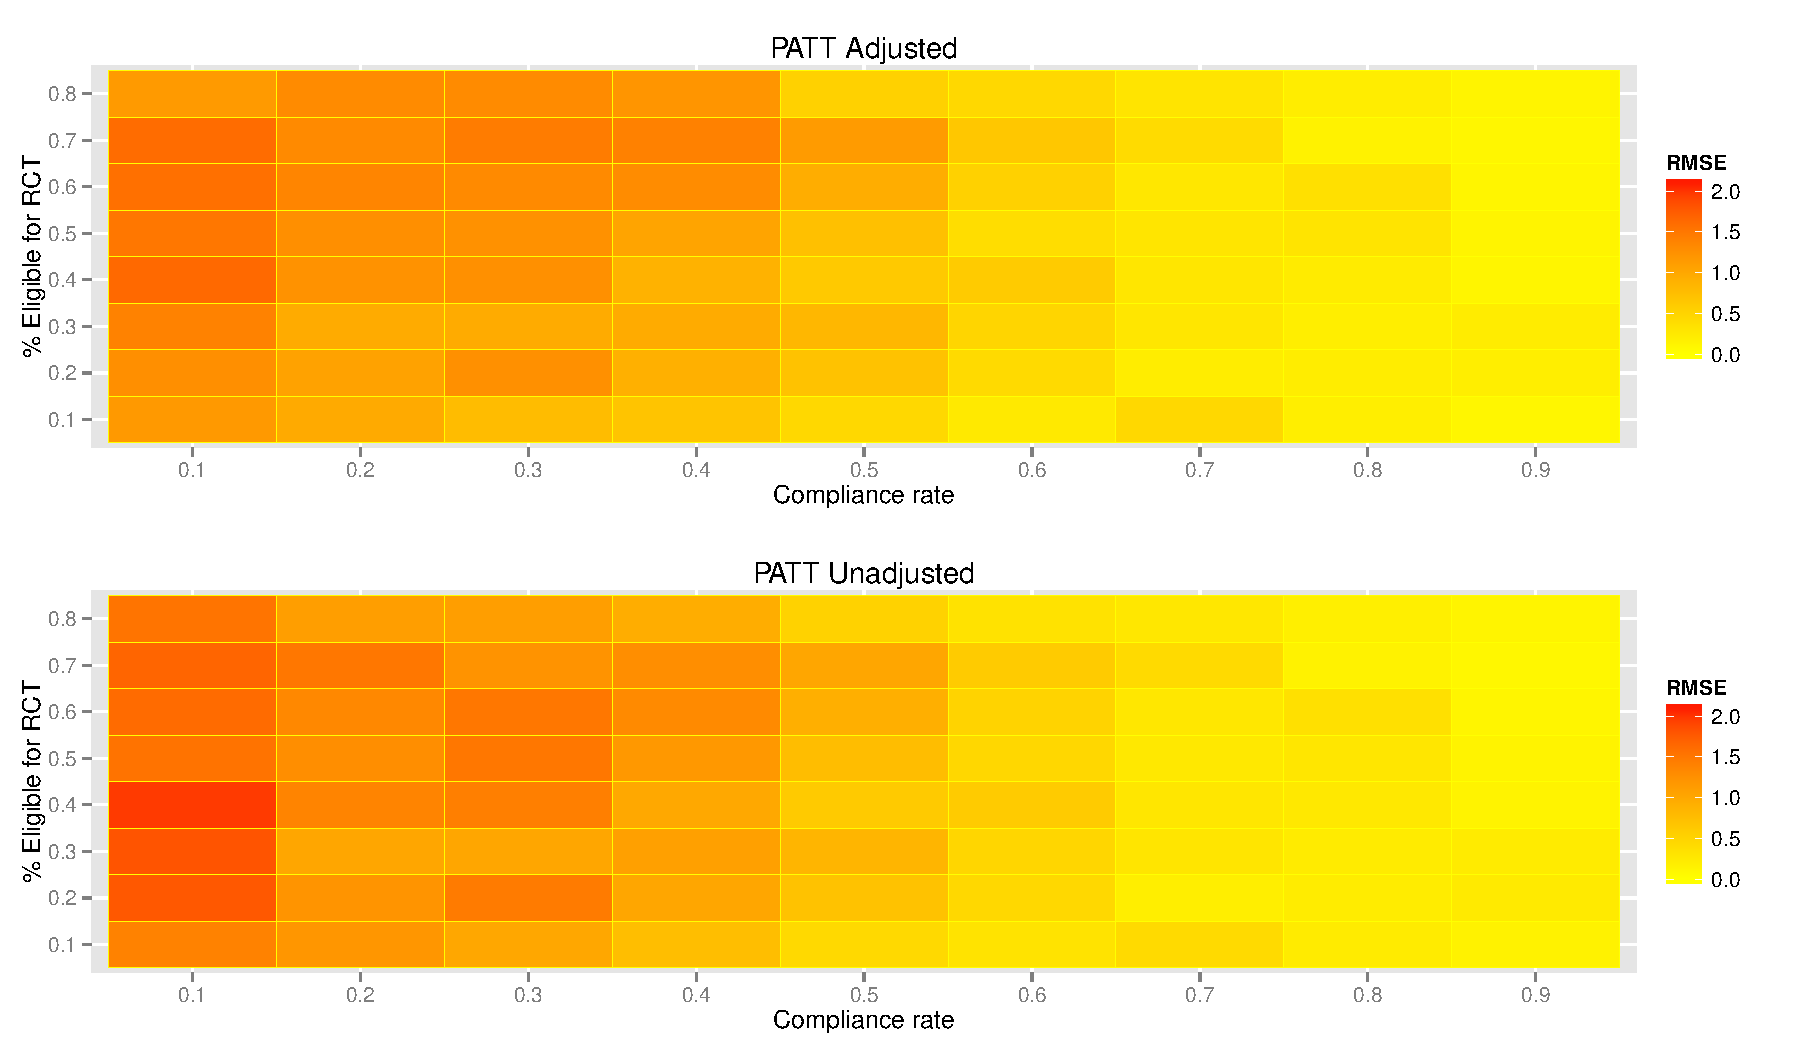
\includegraphics[width = 0.8\textwidth]{mse_ratec_rates_B5}
\caption{Simulation mean squared error, transformed by -$\log$. Darker tiles correspond to lower mean squared error.}
\label{fig:sim_tiles}
\end{center}
\end{figure}


\begin{figure}[htbp]
\begin{center}
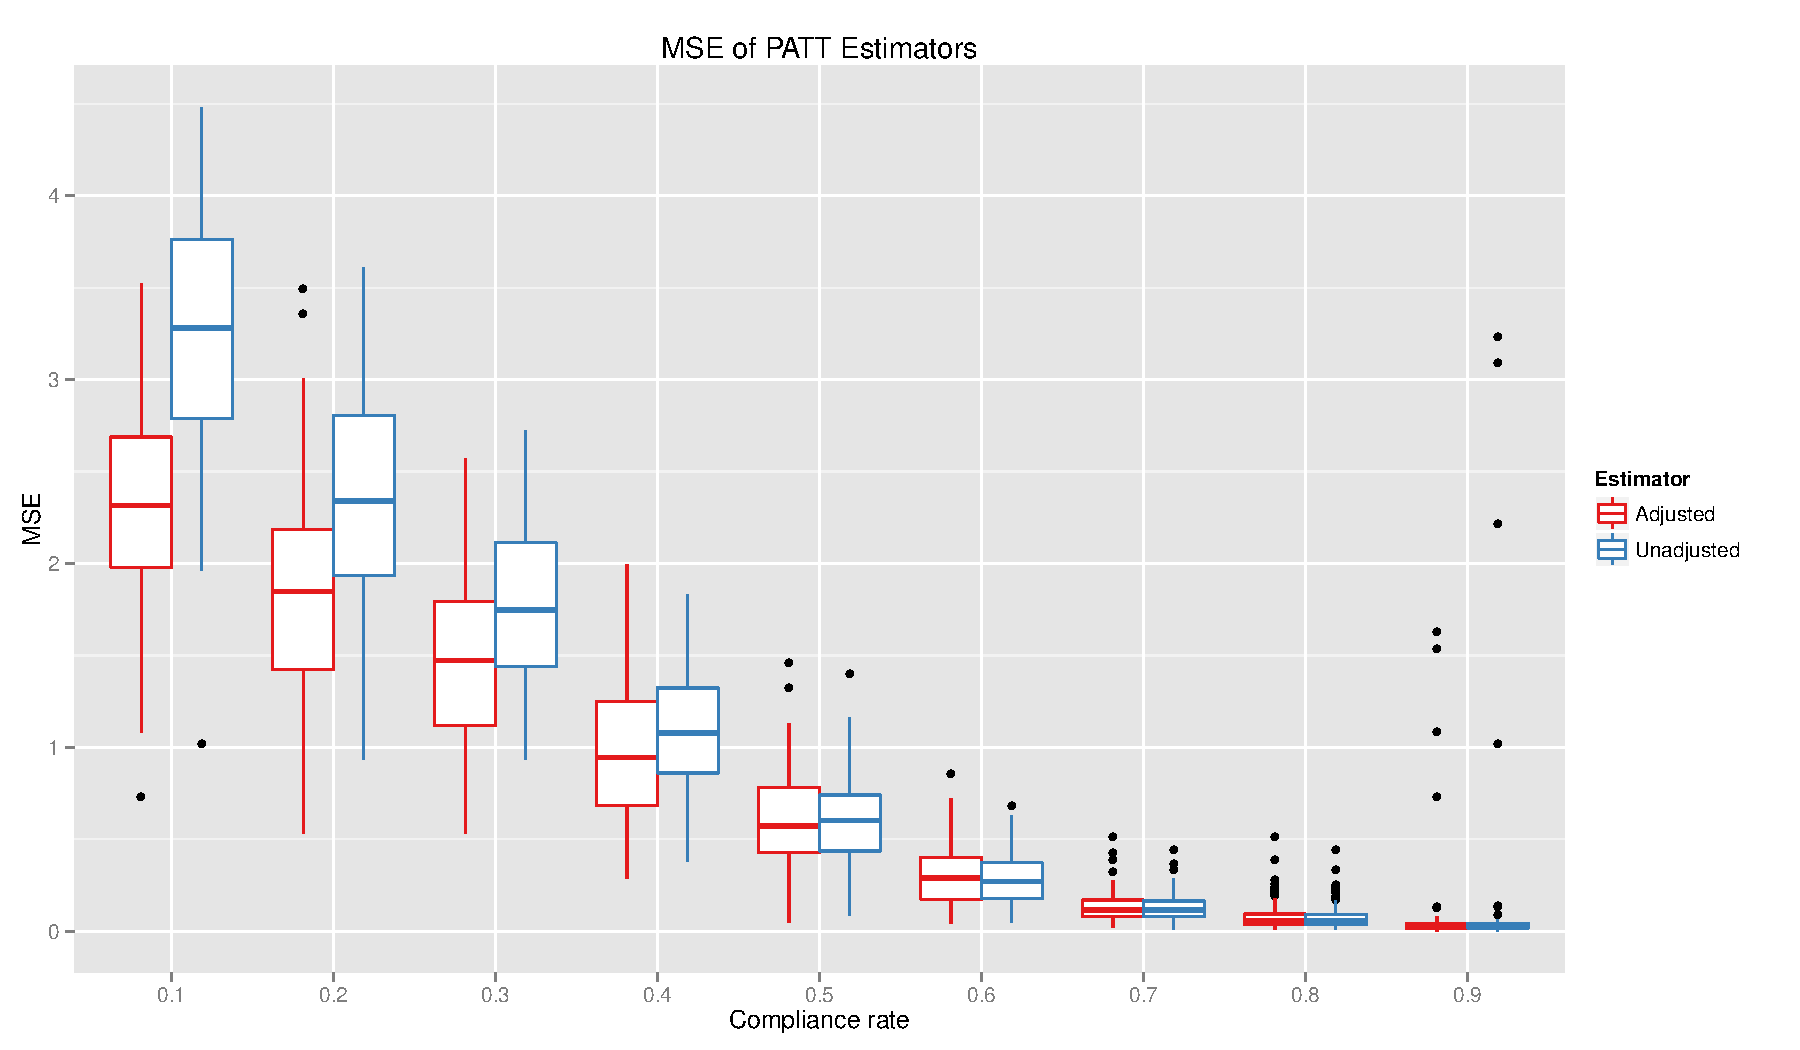
\includegraphics[width = 0.8\textwidth]{mse_boxplots_B5}
\caption{Simulation mean squared error, according to compliance rates in the total population.}
\label{fig:sim_compliance}
\end{center}
\end{figure}
\section{Discussion}

The treatment effect of Medicaid applies to uninsured adults with income below the FPL who express interest in health insurance coverage. The sample population differs in several dimensions from the target population of individuals who will be covered by other Medicaid expansions, such as the Affordable Care Act expansion to cover all adults up to 138\% of the FPL. For instance, the RCT participants are disproportionately white urban--dwellers \cite{Taubman}. The RCT participants volunteered for the study and therefore may be in poorer health compared to the population. \\

\todo{Update tense}
The proposed method allows us to decompose both SATE and PATT estimates by subgroup according to covariates common to both RCT and observational datasets (e.g, demographic variables, pre--existing conditions, and insurance coverage). Since the RCT participants are predominately white and volunteered for the study, we expect to find substantial differences between sample and population estimates in terms of ethnicity and pre--existing condition subgroups. Overall, we expect the PATT estimate to be lower than the SATE estimate due to the adverse selection problem in the RCT. \\

\noindent discuss implications of the simulation results
\begin{itemize}
\item When the rate of crossover from treatment to control is low, the proposed estimator performs better than the estimator which doesn't adjust for non-compliance. 
\item unadjusted is estimating the intention-to-treat effect, which tends to underestimate the average treatment effect on compliers
\item Of course, the simulation results depend on the particular way we parameterized the compliance, selection, treatment assignment, and response schedules.  In particular, the strength of correlation between the covariates and compliance governs how well the estimator will perform.
\item If it is difficult to predict compliance using the observed covariates, then the estimator will perform badly because of noise introduced by incorrectly treating non-compliers as compliers.  Further research should be done into ways to test how well compliance can be predicted.
\end{itemize}


\pagebreak

\begin{singlespace}		%Single-space for bibliography 

%Bibliography
\bibliographystyle{plainnat}
\bibliography{refs}

%Appendix
\pagebreak
\begin{appendices}

\end{appendices}
\end{singlespace}

\itemize
\end{document}


